% !TEX root = ../main.tex
\chapter{評価実験}\label{chap:eval}
% ===== 下書き(Claude、11/20)。レオが読んで理解 → 確認の問い → 直す。納得いかない文は書き換える =====
% 予備審査では予備結果まで。本実験(囲った筐体、実アプリの負荷、OS 標準設定との比較)は 12 月

本章では、提案手法を実機で評価した結果を述べる。評価は次の3つの問いに沿って行った。

\begin{description}
  \item[RQ1] 本研究の対象環境(ラックに並べたノード)で、空間熱干渉はどの程度生じるか。
  \item[RQ2] 提案手法は、別の日のデータに対して 30 秒先の温度をどの程度の誤差で予測でき、その不確かさ $\sigma$ は実際の誤差を表しているか。
  \item[RQ3] 予測に基づくファン制御は、80\,℃ を超えずにファンの稼働をどれだけ減らせるか。また、従来の方式と比べて差があるか。
\end{description}

\section{実験条件}\label{sec:eval-cond}
実験の環境は第\ref{chap:impl}章で述べたとおりである。3台のノード raspi1、raspi2、raspi3 をラック上段に左から並べ、以下ではそれぞれ A、B、C と呼ぶ。B は A のすぐ隣、C は A から2つ離れた位置にある。すべての実験で PoE+ HAT を装着し、ラックは囲わずに開いた状態とした。CPU のガバナは performance に固定し、クロックを 1.8\,GHz とした。

用いたデータを表\ref{tab:eval-data}に示す。パラメータの同定と評価には、異なる日、または同じ日の異なる区間のデータを用いた。同定と評価を同じデータで行うと、モデルがそのデータに合わせ込まれ、誤差を小さく見積もってしまうためである(第\ref{chap:preliminary}章)。

\begin{table}[tb]
  \centering
  \caption{評価に用いたデータ}
  \label{tab:eval-data}
  \small
  \begin{tabular}{llp{0.32\linewidth}p{0.22\linewidth}}
    \toprule
    名前 & 日時 & 内容 & 用途 \\
    \midrule
    ステップ & 11/13 昼(約2時間) & A の負荷とファンを段階的に切り替え & A の同定(別の日) \\
    ランダム & 11/14 夜(約5.4時間) & 3台の負荷とファンを独立にランダムに切り替え & 前半で同定、後半で予測の評価 \\
    比較 & 11/14〜15 夜(約8.1時間) & 5条件 × 3巡 × 3台のファン制御 & 制御の評価(RQ3) \\
    \bottomrule
  \end{tabular}
\end{table}

モデルの時間刻みは $\Delta t = 5$ 秒とし、1秒ごとの計測値の5秒平均を用いた。温度は室温からの上昇分 $\theta = T - T_{\mathrm{amb}}$ で扱った。室温はラックから離れた位置の SwitchBot ハブ2 の値とした。ランダムの実験では室温が 21.1\,℃ から 19.7\,℃ まで、比較の実験では 22.0〜22.6\,℃ の範囲で変化した。

\section{熱干渉の大きさ(RQ1)}\label{sec:eval-interference}
第\ref{chap:preliminary}章で、ラックと机の上の両方で、A だけに負荷をかけても B の温度上昇は C と同じ約 0.4〜0.5\,℃ であり、干渉がほぼ見えないことを示した。ここでは、ランダムの実験から同定した干渉の係数 $c$ で、この結果を確かめる。

ランダムの実験の前半から式(\ref{eq:full})のパラメータを同定した結果を表\ref{tab:eval-identify}に示す。$c$ は隣のノードの温度が定常的に 1\,℃ 上がったとき、自ノードの温度が何度上がるかに対応する量である。B の $c$ は 0.0071 で、隣が 1\,℃ 上がっても自ノードは定常で約 0.08\,℃ しか上がらない。A と C の $c$ は負になった。隣の排熱で自ノードが冷えることは物理的にありえないため、これは前半のデータに偶然あった相関を拾ったものと考えられる。実際、ランダムの実験では3台の負荷を独立に決めており、隣の温度と自ノードの温度の間に因果関係はない。

以上より、本研究の対象環境では空間熱干渉はほぼ生じない。以降の評価では $c \geq 0$ の制約を設け、A と C では $c = 0$ とした。

\begin{table}[tb]
  \centering
  \caption{ランダムの実験の前半から同定したパラメータ(制約なし)}
  \label{tab:eval-identify}
  \begin{tabular}{lrrrrr}
    \toprule
    ノード & $a$ & $\tau$ [s] & $b$ & $e$ & $c$ \\
    \midrule
    A & 0.949 & 96 & 1.42 & $-1.04$ & $-0.0135$ \\
    B & 0.911 & 54 & 1.96 & $-1.16$ & $0.0071$ \\
    C & 0.939 & 80 & 1.58 & $-1.10$ & $-0.0027$ \\
    A(11/13 のステップ) & 0.927 & 66 & 1.92 & $-1.41$ & --- \\
    \bottomrule
  \end{tabular}
\end{table}

\section{予測精度(RQ2)}\label{sec:eval-predict}
\subsection{方法}
ランダムの実験の後半を用いて、30 秒先($m = 6$ ステップ先)の温度の予測誤差を求めた。比較した手法は次の3つである。

\begin{itemize}
  \item Self-only:自ノードの熱モデル(式(\ref{eq:self-fan}))で、現在の実測値から 30 秒先まで計算する
  \item KF(H なし):式(\ref{eq:self-fan})を状態方程式とするカルマンフィルタ
  \item KF + H(提案):外部熱影響 $H$ を状態に含めたカルマンフィルタ(第\ref{chap:method}章)
\end{itemize}

いずれの手法も、30 秒先までの負荷とファンの状態は現在の値のまま変わらないと仮定する。第\ref{chap:preliminary}章で述べたとおり、先行発表では未来の実測値を予測に用いていたが、実際の制御では未来の値は分からないため、本研究では用いない。

30 秒の間に負荷かファンが切り替わると、この仮定が成り立たない。そこで評価区間を、30 秒の間に切り替えがない「入力一定」の区間(全体の 89\%)と、切り替えをまたぐ区間(11\%)に分けて誤差を求めた。

\subsection{結果}
平均絶対誤差(MAE)を表\ref{tab:eval-mae}に示す。入力一定の区間では、3台とも 30 秒先を MAE 約 0.7\,℃ で予測できた。一方、切り替えをまたぐ区間の MAE は約 4\,℃ で、全体の誤差の大半はこの 11\% の区間から生じている。これは未来の負荷を知らないことによる誤差であり、どの手法でも避けられない。

図\ref{fig:eval-predict}に、評価区間の一部(A)の実測と 30 秒先の予測を示す。負荷とファンが変わらない間は、予測は実測に沿う。一方、負荷やファンが切り替わった直後は、予測が実測から最大で数℃ずれ、30 秒遅れて追いつく。予測 + マージンの帯の幅は時間によらず一定である(後述)。

\begin{figure}[tb]
  \centering
  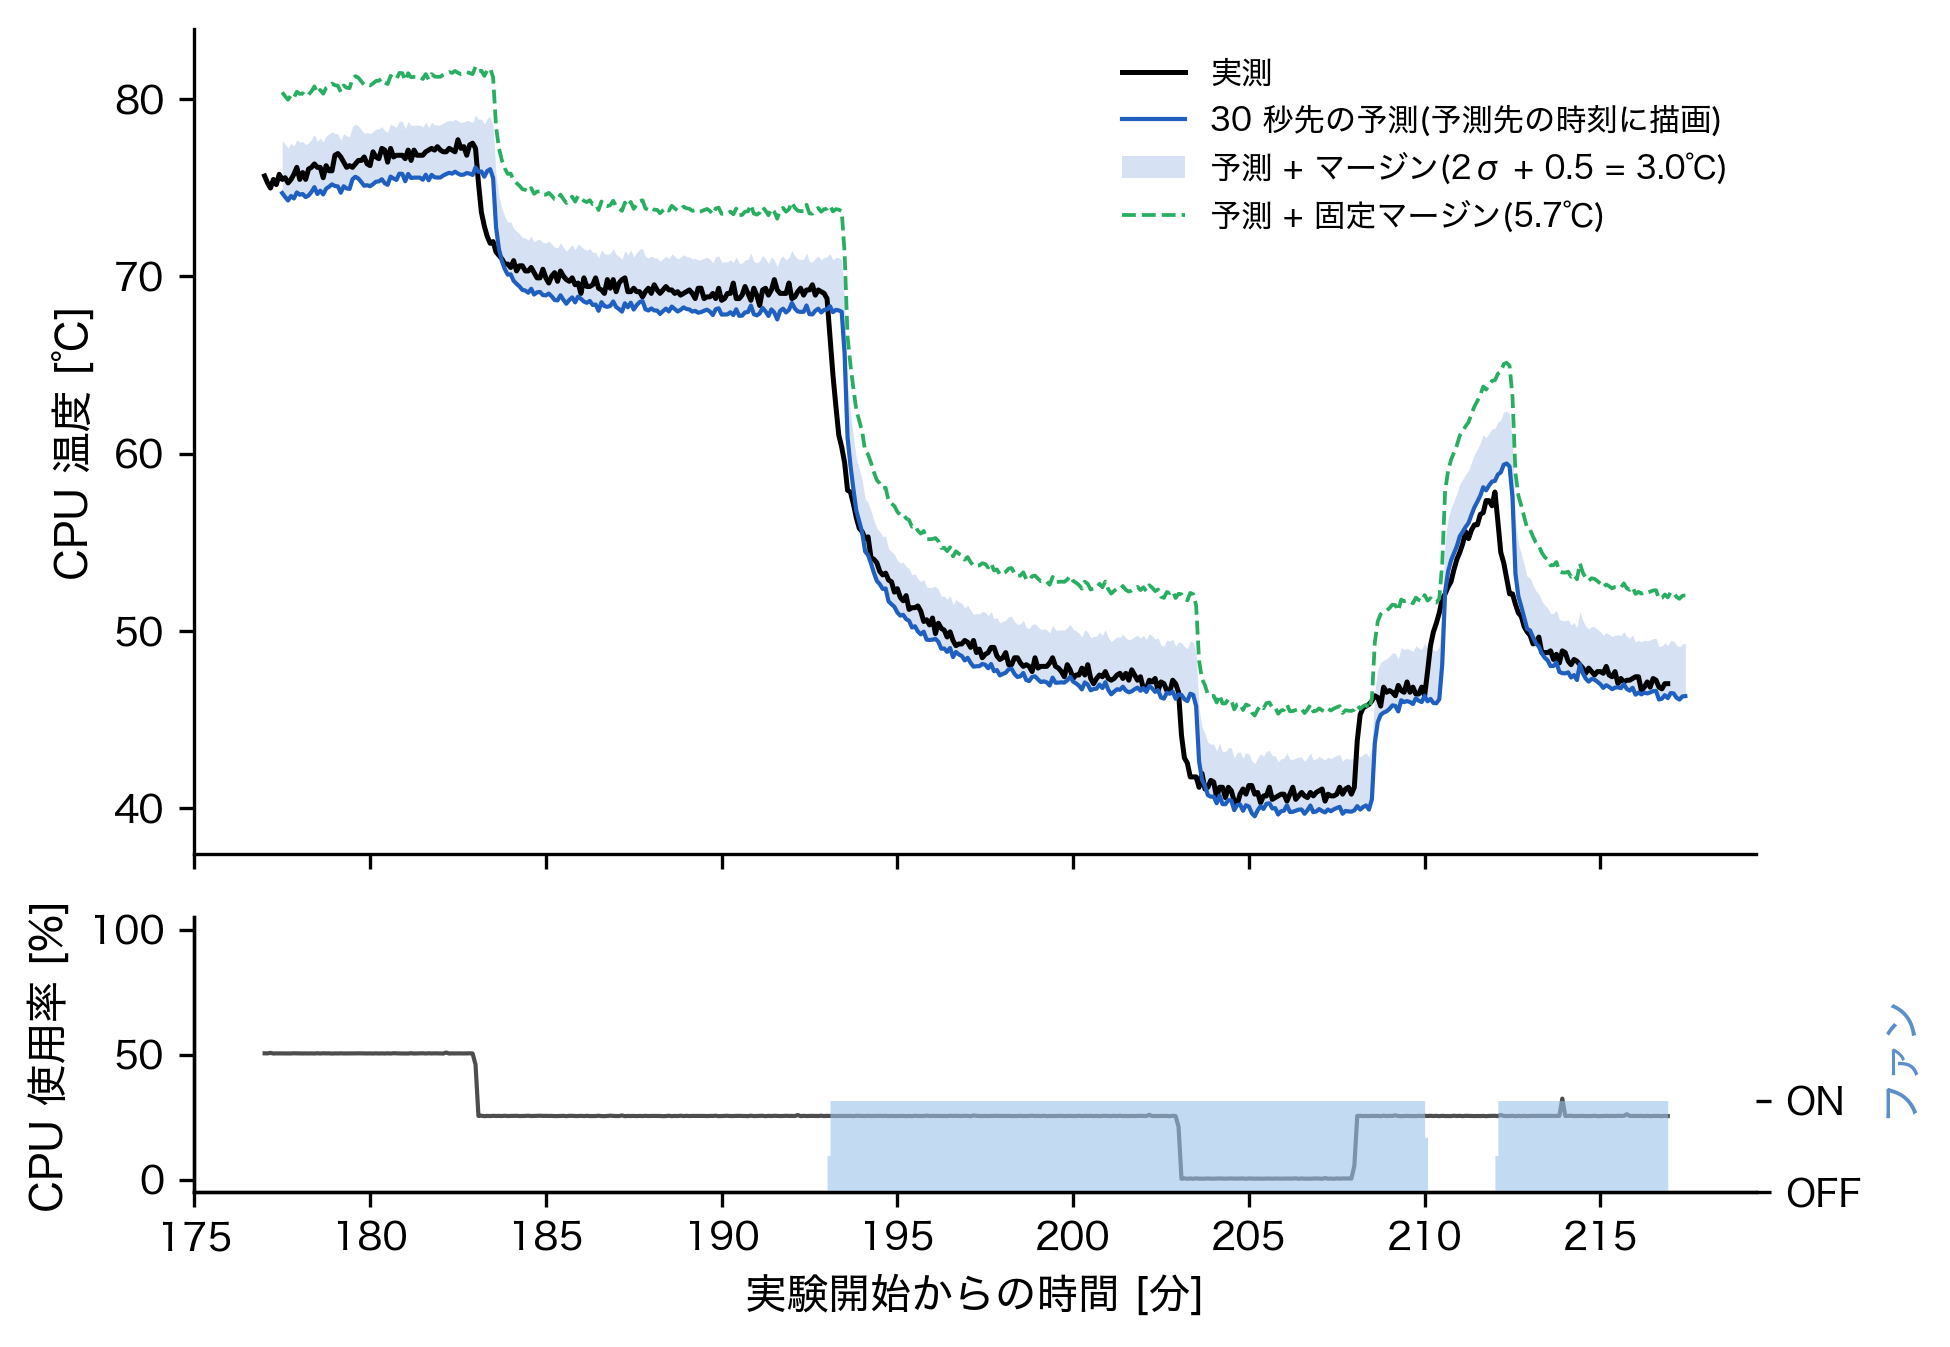
\includegraphics[width=\linewidth]{fig_predict.png}
  \caption{ランダムの実験の後半(同定に使っていない区間)の A の温度と 30 秒先の予測。予測は、予測した先の時刻(30 秒後)の位置に描いた。下は CPU 使用率とファンの状態}
  \label{fig:eval-predict}
\end{figure}

KF(H なし)と Self-only の誤差はほぼ同じであった。また、比較のため、負荷やファンの入力を使わず温度の履歴だけから予測する自己回帰(AR)モデル(先回りの熱管理の研究\cite{coskun2008proactive}で用いられた種類の予測)も評価した。温度の差分の AR モデルを前半で同定すると、後半の入力一定の区間の MAE は A で 0.72\,℃、B で 0.65\,℃、C で 0.64\,℃ となり、物理モデル(Self-only)の 0.70、0.78、0.68\,℃ とほぼ同じであった。B では、後述するモデルのずれのために、AR の方が小さかった。単に 30 秒先の温度を当てるだけであれば、このデータでは物理モデルの利点は小さい。ただし、ファンの判断に必要なのは「この先ファンを OFF にしておいたら何℃になるか」という入力を仮定した予測であり、入力を持たない AR モデルではこれを求められない。物理モデルを用いる意味はこの点にある。A の KF + H は他の手法より誤差が大きい(入力一定で 1.12\,℃)。これは前節で述べた負の $c$ によるもので、前半の偶然の相関が後半では成り立たないためである。$c \geq 0$ の制約を入れると、A の KF + H は H なしと同じになる。

別の日(11/13 のステップの実験)に同定したパラメータで A を予測すると、入力一定の区間の MAE は 0.70\,℃ から 1.05\,℃ に増え、予測が実測より低めに偏った。時定数も 66 秒と 96 秒で異なる。日によって室温やラック内の空気の状態が変わるためと考えられ、運用では定期的にパラメータを同定し直す必要があることを示している。

\begin{table}[tb]
  \centering
  \caption{30 秒先の予測の平均絶対誤差(ランダムの実験の後半)[℃]}
  \label{tab:eval-mae}
  \begin{tabular}{llrrr}
    \toprule
    ノード & 手法 & 全区間 & 入力一定 & 切り替え \\
    \midrule
    A & Self-only & 1.05 & 0.70 & 3.94 \\
    A & KF(H なし) & 1.07 & 0.71 & 3.94 \\
    A & KF + H & 1.46 & 1.12 & 4.20 \\
    B & Self-only & 1.16 & 0.78 & 4.18 \\
    B & KF + H & 1.18 & 0.81 & 4.15 \\
    C & Self-only & 1.04 & 0.68 & 3.94 \\
    C & KF + H & 1.07 & 0.71 & 3.95 \\
    A(11/13 の値) & Self-only & 1.37 & 1.05 & 3.99 \\
    \bottomrule
  \end{tabular}
\end{table}

\subsection{不確かさ $\sigma$ とマージン}
予測にマージンを足した値を実測が上回った割合(超過率)を表\ref{tab:eval-margin}に示す。$\alpha = 2$ のとき、誤差が正規分布に従い $\sigma$ が正しければ、超過率は約 2.3\% になるはずである。比較のため、同定データの誤差の 97.7\% 分位点を固定マージンとする方式(Self-only + 固定)も示す。

提案手法の $\sigma$ は時間によらずほぼ一定(A 1.19、B 0.94、C 0.99\,℃)となった。式(\ref{eq:adaptive-q})の適応的なプロセスノイズは $H$ にだけ加わり、$c$ を通してしか温度に影響しない。干渉がない($c \approx 0$)と、$\sigma$ はカルマンフィルタの定常値に収束する。したがって本研究の環境では、提案手法の「動的マージン」は実質的に一定のマージンとなる。

マージンの平均は、提案手法が 2.4〜2.9\,℃ で、固定マージン(3.6〜5.7\,℃)の約半分である。超過率は、入力一定の区間では 0.5〜5.9\% で目標に近いが、切り替えの区間では 21〜34\% と大きい。$\sigma$ は負荷が急に変わることによる不確かさを含んでいない。固定マージンは切り替えの誤差も含めて決めるため、超過率は 1〜2\% に収まるが、その分マージンが大きい。

\begin{table}[tb]
  \centering
  \caption{マージンと超過率(ランダムの実験の後半)}
  \label{tab:eval-margin}
  \begin{tabular}{llrrrr}
    \toprule
    & & 平均マージン & \multicolumn{3}{c}{超過率 [\%]} \\
    \cmidrule(lr){4-6}
    ノード & 手法 & [℃] & 全区間 & 入力一定 & 切り替え \\
    \midrule
    A & Self-only + 固定 & 5.68 & 1.1 & 0.0 & 10 \\
    A & 提案 & 2.89 & 3.7 & 0.7 & 27 \\
    B & Self-only + 固定 & 5.22 & 2.2 & 0.1 & 19 \\
    B & 提案 & 2.38 & 9.0 & 5.9 & 34 \\
    C & Self-only + 固定 & 3.56 & 2.2 & 0.1 & 19 \\
    C & 提案 & 2.48 & 2.8 & 0.5 & 21 \\
    \bottomrule
  \end{tabular}
\end{table}

\section{ファン制御(RQ3)}\label{sec:eval-control}
\subsection{方法}
次の5つの条件でファンを制御し、比べた。

\begin{itemize}
  \item ファンなし:ファンを回さない(ただし 82\,℃ 以上ではノード側の強制 ON が働く。\ref{sec:impl-fan}節)
  \item 常時 ON:ファンを回し続ける
  \item しきい値:75\,℃ 以上で ON、70\,℃ 以下で OFF
  \item Self-only + 固定:Self-only の 30 秒先予測が $80 - M_{\mathrm{fix}}$ を超えたら ON。$M_{\mathrm{fix}}$ は前節の固定マージン(A 4.87、B 4.99、C 3.50\,℃)
  \item 提案:カルマンフィルタの 30 秒先予測が $T_{\mathrm{safe}} = 80 - (\alpha\sigma + \delta)$ を超えたら ON($\alpha = 2$、$\delta = 0.5$\,℃)
\end{itemize}

予測を用いる2つの方式では、ファンを止めたまま 30 秒後の温度を予測し、それが安全閾値を超えるときに ON とした。OFF にするのは、ON にしてから 30 秒以上たち、予測が安全閾値より 1\,℃ 以上低くなったときである(\ref{sec:method-control}節)。制御器のパラメータは、ランダムの実験の全データから $c = 0$ として同定した。

負荷は、20 分の中で 1〜4 コアの負荷と休みを組み合わせたパターンとした(4 コアの負荷を含む)。3台に同じ条件・同じ負荷を同時にかけ、5条件を1巡として3巡行った。各巡の条件の順番はランダムにし、条件の間には 12 分の休みを入れて温度を戻した。各条件の開始時の温度は 57.1〜57.7\,℃ でそろっていた。各条件のデータは 3巡 × 3台 = 9 回である。

評価指標は、ファン稼働率(ファンが ON だった時間の割合)、最高温度、80\,℃ を超えた時間、スロットリングの時間、強制 ON の時間、ON にした回数とした。

\subsection{結果}
結果を表\ref{tab:eval-control}と図\ref{fig:eval-bars}に、1巡目のノード A の温度とファンの時系列を図\ref{fig:eval-control}に示す。

\begin{figure}[tb]
  \centering
  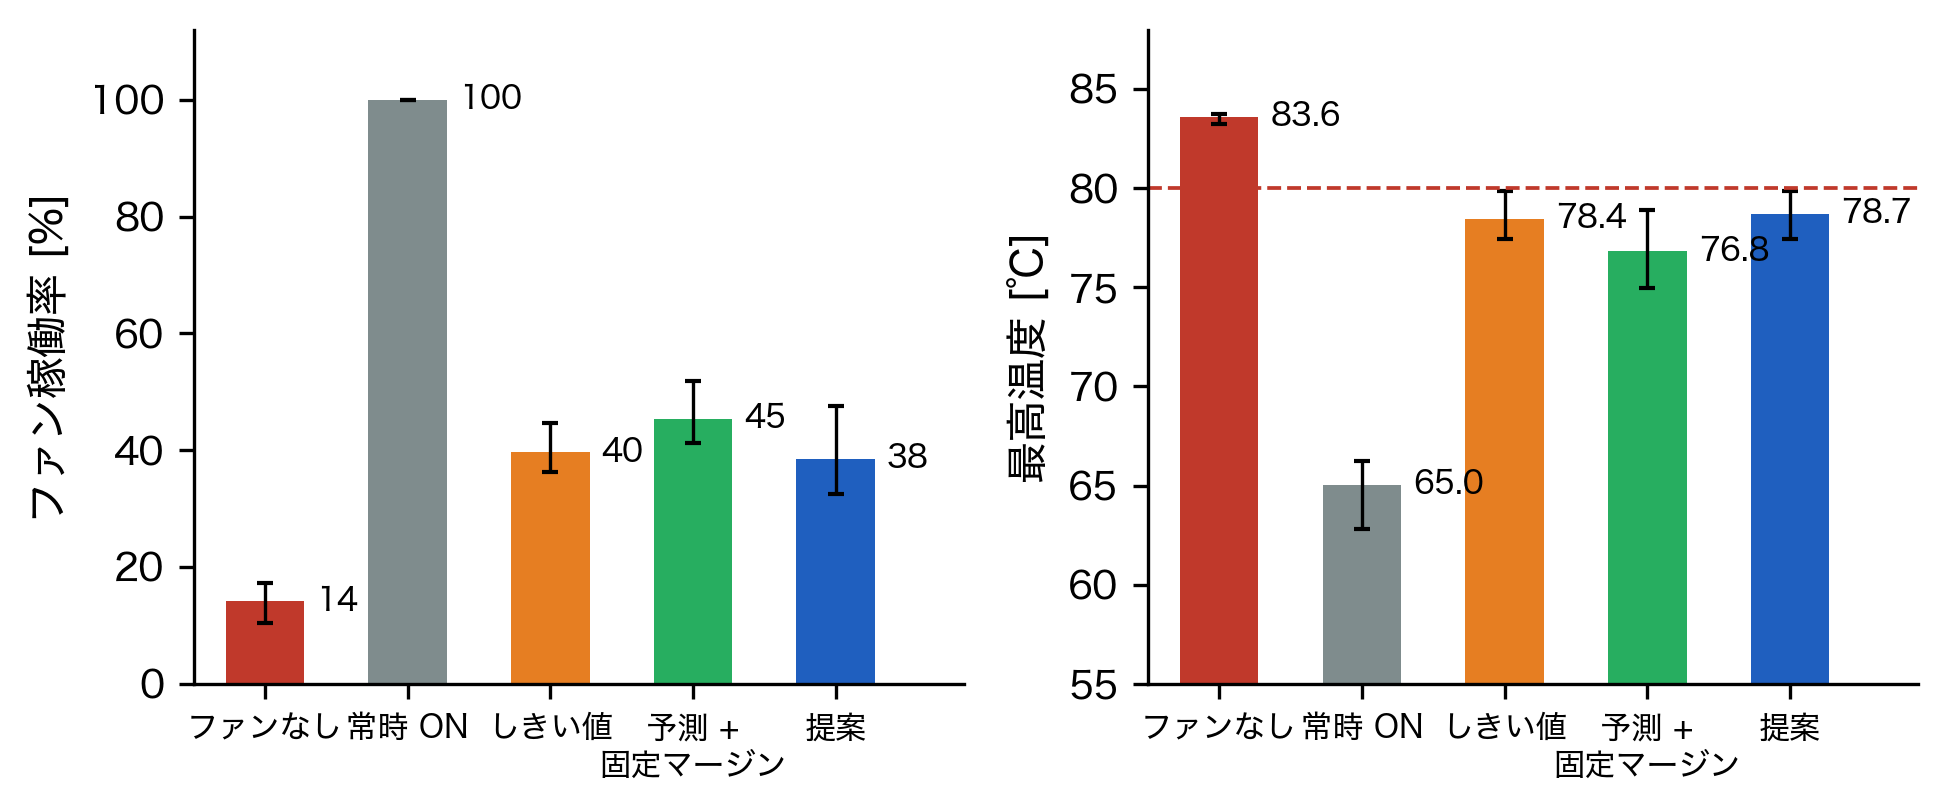
\includegraphics[width=\linewidth]{fig_control_bars.png}
  \caption{各条件のファン稼働率と最高温度(9 回の平均。ひげは最小と最大)}
  \label{fig:eval-bars}
\end{figure}

\begin{table}[tb]
  \centering
  \caption{ファン制御の比較(各条件 9 回の平均。20 分あたり)}
  \label{tab:eval-control}
  \small
  \begin{tabular}{lrrrrr}
    \toprule
    条件 & 稼働率 & 最高温度 [℃] & 80\,℃ 超過 [s] & スロットリング [s] & ON の回数 \\
    \midrule
    ファンなし & 14\%$^{*}$ & 83.6 & 696 & 165 & 159 \\
    常時 ON & 100\% & 65.0 & 0 & 0 & 1 \\
    しきい値(75/70\,℃) & 40\% & 78.5 & 0 & 0 & 15.0 \\
    Self-only + 固定 & 45\% & 76.8 & 0 & 0 & 17.8 \\
    提案 & 38\% & 78.7 & 0 & 0 & 15.7 \\
    \bottomrule
    \multicolumn{6}{l}{\footnotesize $^{*}$ 82\,℃ 以上での強制 ON のみ}
  \end{tabular}
\end{table}

\begin{figure}[tb]
  \centering
  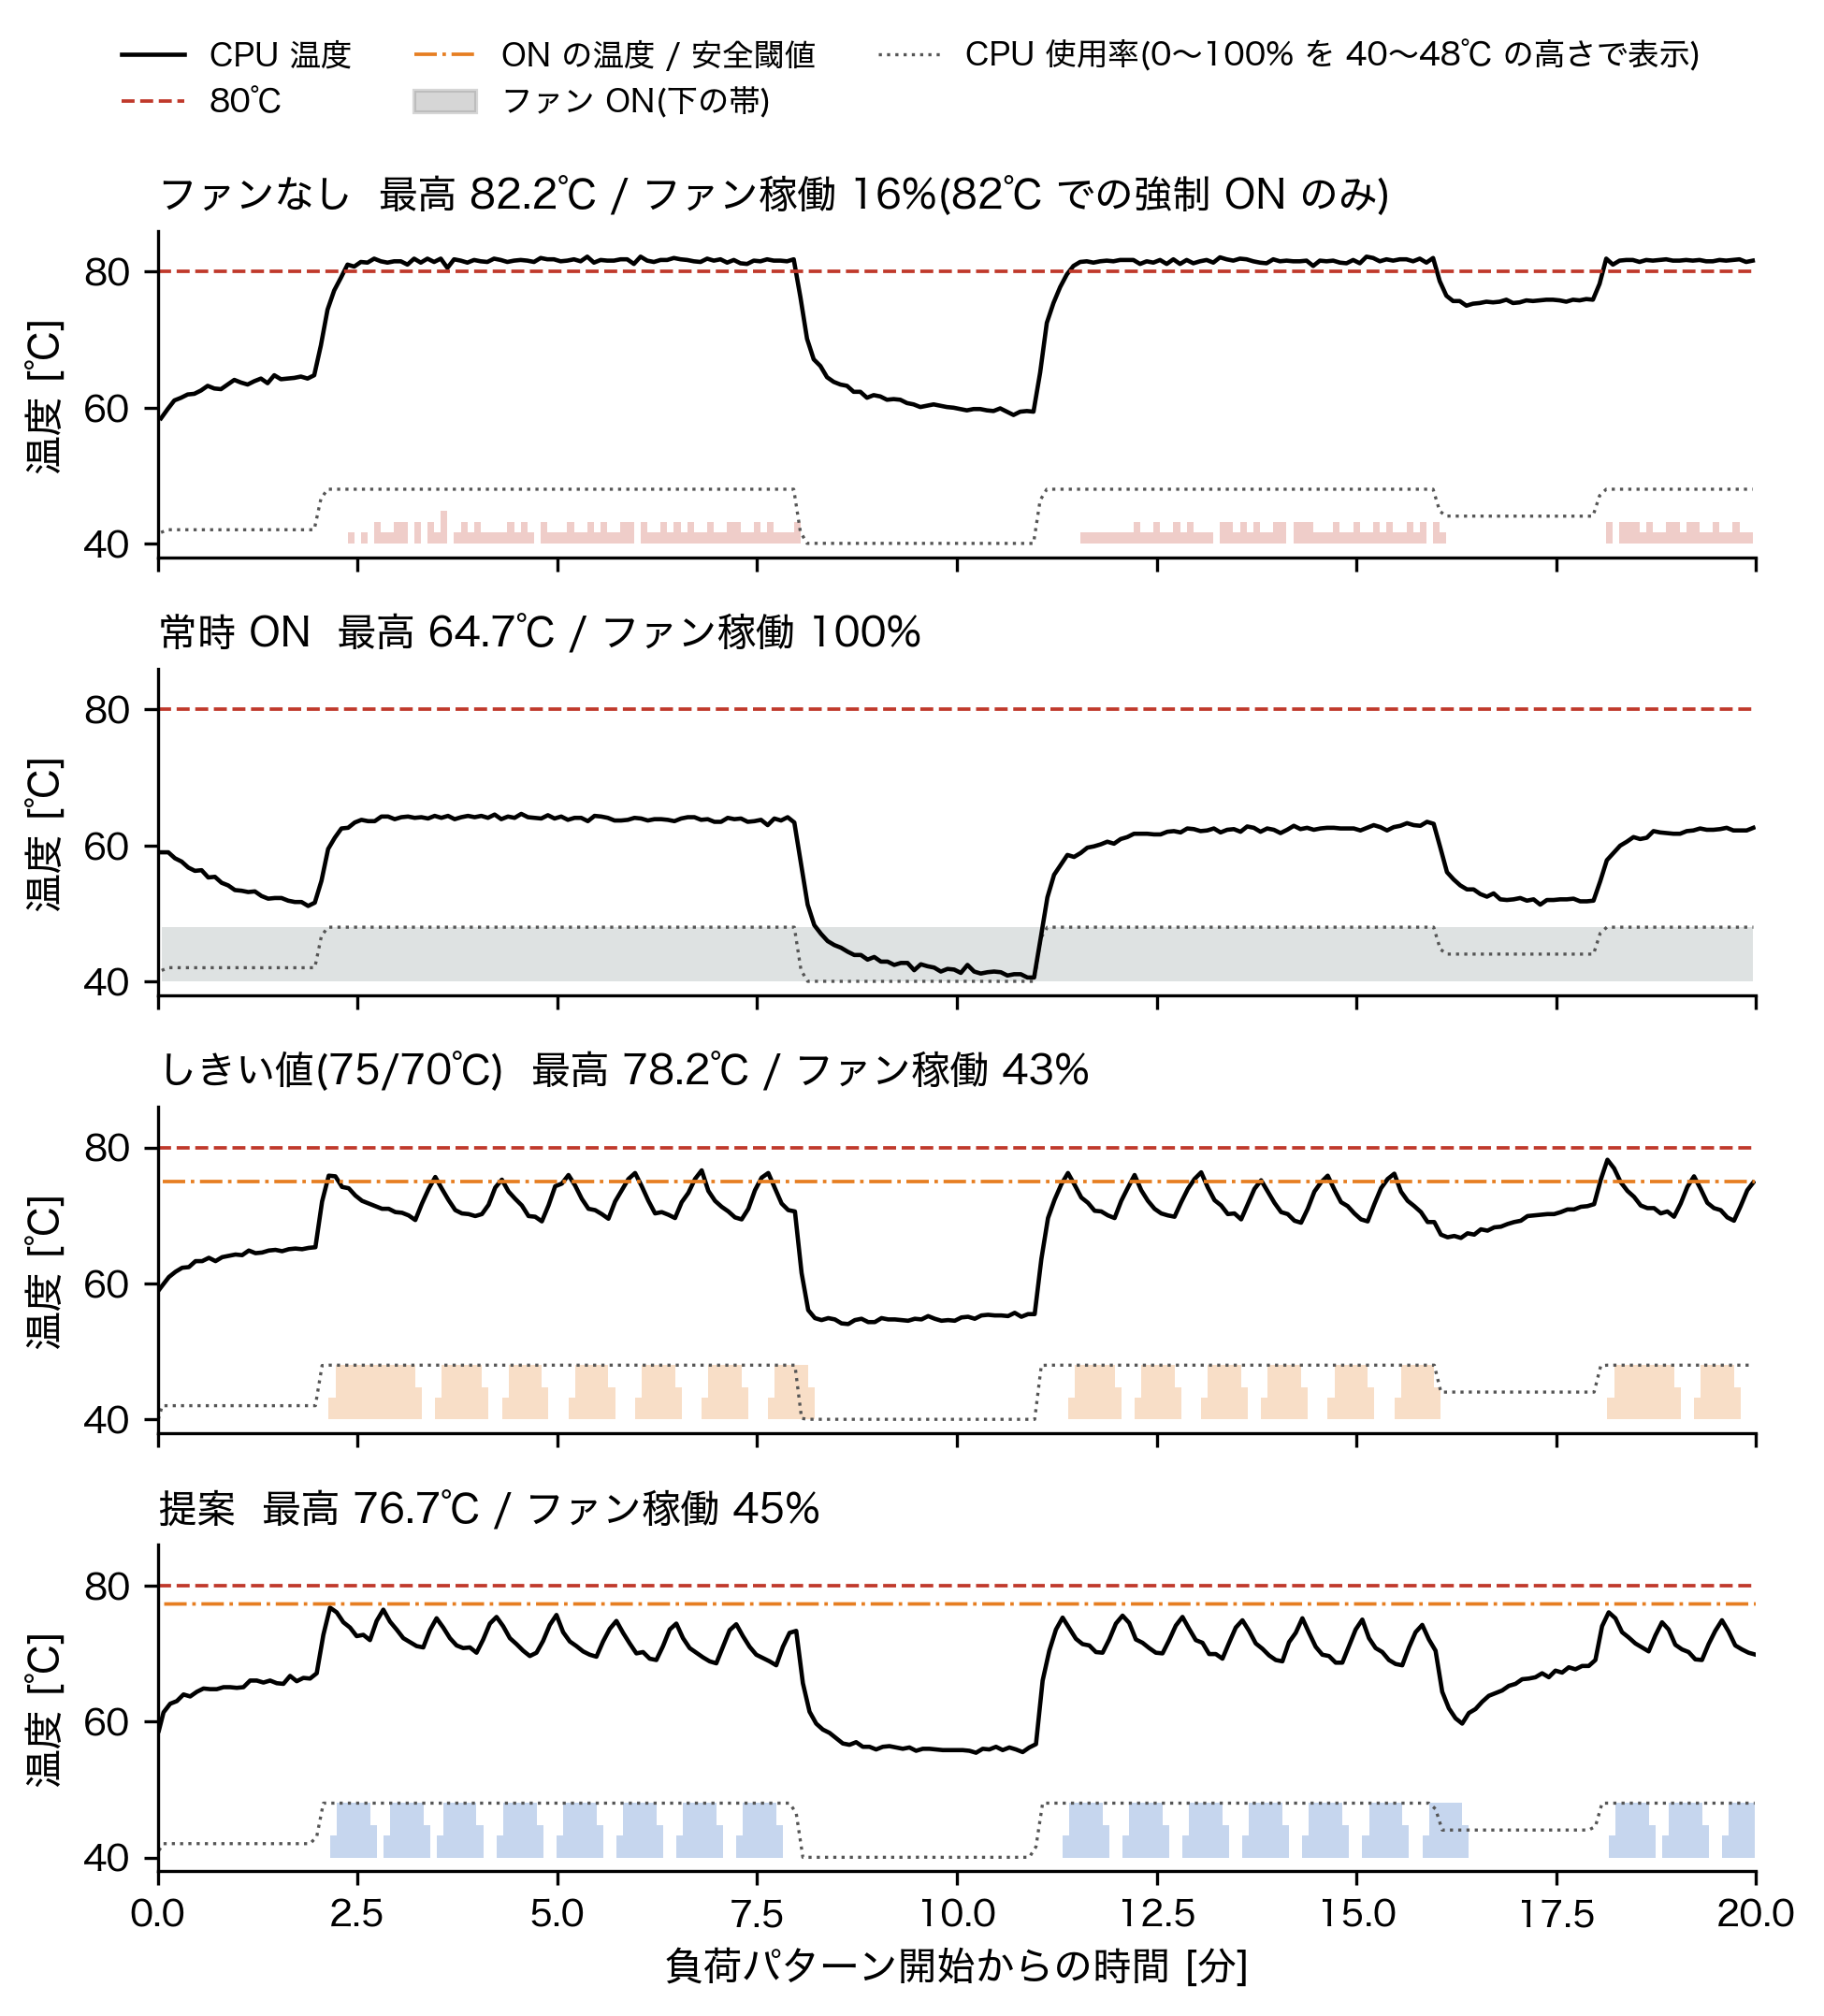
\includegraphics[width=\linewidth]{fig_control_round.png}
  \caption{ファン制御の比較実験の時系列(1巡目、ノード A。各条件 20 分の負荷パターン)}
  \label{fig:eval-control}
\end{figure}

予測を用いる2つの方式としきい値方式は、いずれも 80\,℃ を超えず、スロットリングと強制 ON も一度も起きなかった。ファン稼働率は 38〜45\% で、常時 ON と比べて稼働を 55〜62\% 減らした。ファンなしでは、20 分のうち約 11.6 分 80\,℃ を超え、約 2.7 分スロットリングが起きた。

一方、提案手法としきい値方式の差はほぼなかった(稼働率 38\% と 40\%、最高温度 78.7\,℃ と 78.5\,℃)。ノード別のファン稼働率(提案/しきい値)は A 45.6/43.6\%、B 32.5/37.0\%、C 37.4/38.3\% で、ノードによって大小が入れ替わり、一貫した差はない。Self-only + 固定は、固定マージンが提案手法のマージンより大きい分、最高温度が低く(76.8\,℃)、稼働率が高い(45\%)。

\section{設定を変えたときの比較(シミュレーション)}\label{sec:eval-sim}
前節の比較は、各方式の設定(しきい値の温度、マージンの大きさ)を1つずつ選んだ結果である。設定を変えれば結果も変わるため、1点の比較だけでは方式の優劣は言えない。そこで、シミュレーションで設定を広く変え、ファン稼働率と最高温度の関係を曲線として比べた。

実機の代わりとなるモデルには 11/13 のステップの実験で同定した A のパラメータを、制御器にはランダムの実験で同定したパラメータを用いた。異なるデータで同定したモデルどうしにすることで、制御器のモデルが実機と完全には一致しない状況を再現した。プロセスノイズと観測ノイズは実験から求めた値とし、乱数の系列は全方式で同じにした。負荷は比較実験と同じパターンと、ランダムなパターン3本(各3時間)を用いた。動かした設定は、しきい値方式の ON の温度 60〜79\,℃、固定マージン 0〜8\,℃、提案手法の $\alpha$ 0〜5 である。

結果を図\ref{fig:eval-sim}に示す。3つの方式の曲線はほぼ重なった。同じ最高温度で比べると、予測を用いる方式はしきい値方式より稼働率が数ポイント低い程度である。提案手法と Self-only + 固定は、$\sigma$ が一定であるためほぼ同じ曲線になった。曲線上のどこに来るかは方式よりも設定、つまり 80\,℃ にどこまで近づけるかで決まる。この結果は実機の比較と一致する。

\begin{figure}[tb]
  \centering
  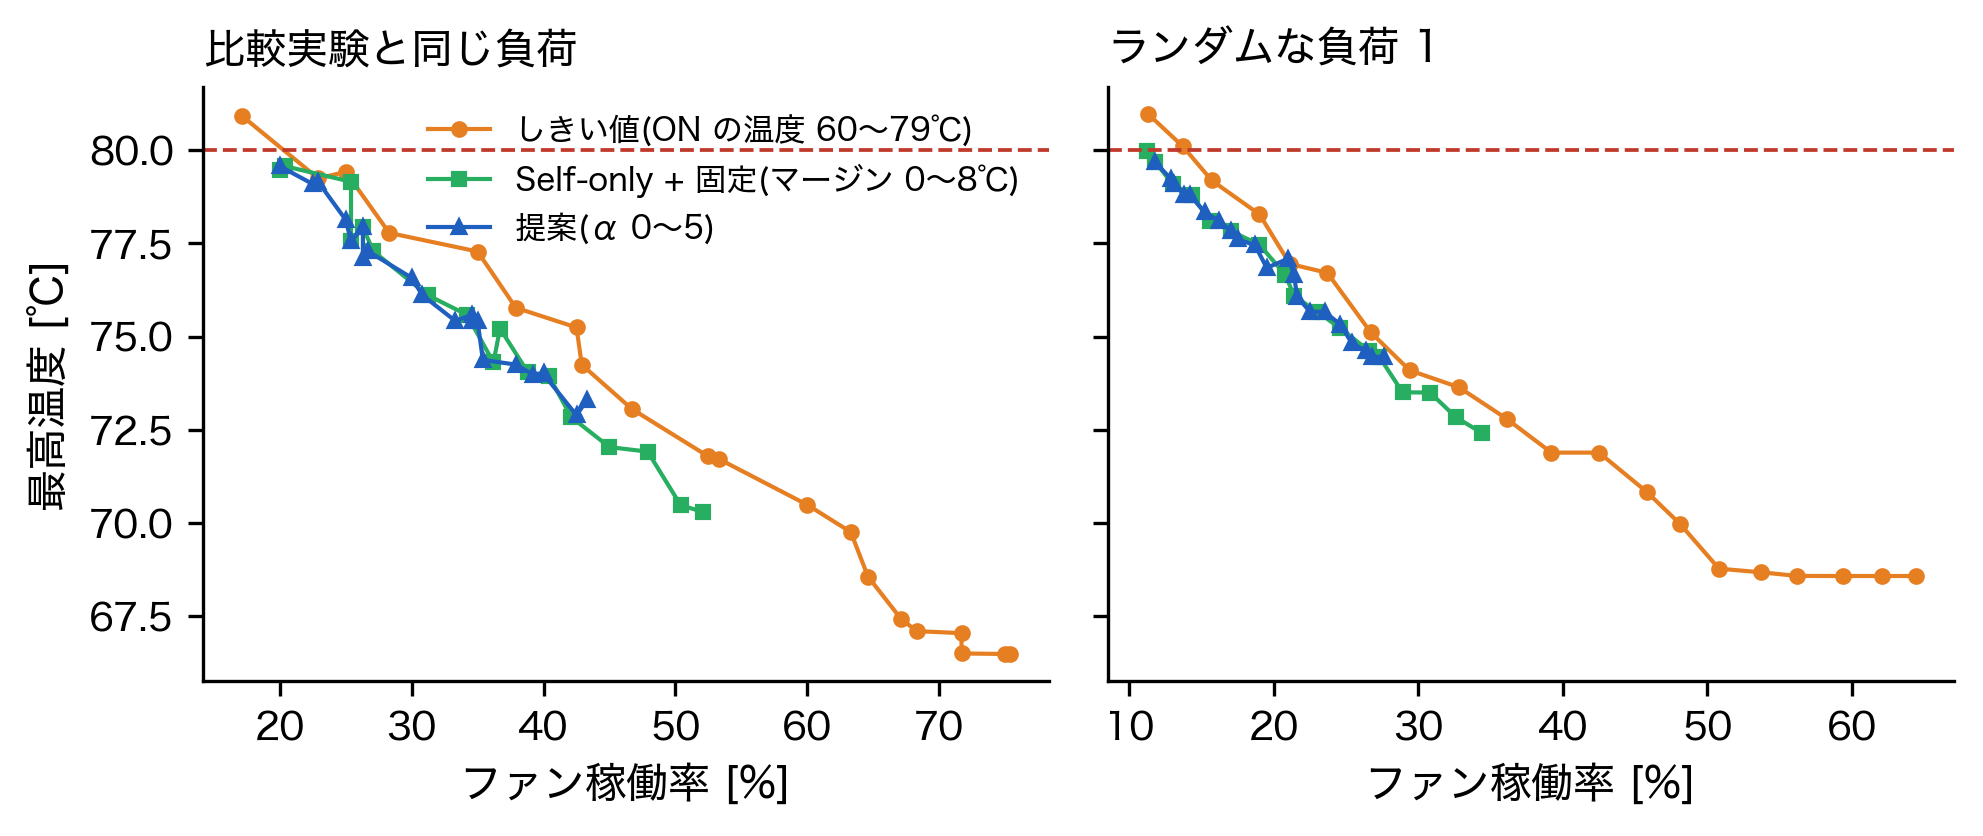
\includegraphics[width=\linewidth]{fig_tradeoff.png}
  \caption{設定を変えたときのファン稼働率と最高温度の関係(シミュレーション。左:比較実験と同じ負荷、右:ランダムな負荷の1本)}
  \label{fig:eval-sim}
\end{figure}

\section{冷却の効きを遅くしたときの比較(シミュレーション)}\label{sec:eval-slow}
PoE+ HAT のファンは、ON にしてから 5 秒以内に温度が下がり始める。予測を用いる方式としきい値方式に差がなかったのは、この効きの速さのためである可能性がある。そこで、前節のシミュレーションに冷却の効きの遅れを加え、遅れによって方式の差がどう変わるかを調べた。条件は結果を見る前に決めて記録した。

遅れは2種類とした。1つ目はむだ時間 $L$ で、ファンの指令が $L$ 秒後に効き始める(0, 15, 30, 60, 90, 120 秒)。2つ目は1次遅れで、冷却の効きが時定数 $\tau_f$ でゆっくり立ち上がり、ゆっくり下がる(0, 30, 60, 120, 240 秒)。部屋の空調のような冷却は後者に近い。冷却の強さ(係数 $e$)は変えていない。予測を用いる方式は遅れを知っているとし、先読みを $30 + L$ 秒(または $30 + \tau_f$ 秒)に延ばした。判断は前節までと同じく「今からファンを OFF にしておいたら、先読みの間に安全閾値を超えるか」である。設定は前節より広く動かし(しきい値 40〜79\,℃、固定マージン 0〜20\,℃、$\alpha$ 0〜12)、各条件で 80\,℃ を超えない設定のうち最も少ない稼働率(最小稼働率)を比べた。予測を用いる方式の最小稼働率がしきい値方式より 5 ポイント以上低い場合を「予測が有効」と判定した。

結果を図\ref{fig:eval-slow}に示す。むだ時間では、遅れが大きくなるほど差が開いた。遅れ 0 では差は 1〜5 ポイントで、どのパターンでも有効とは判定されなかった。15 秒では 4 パターン中 2 本、30 秒では 4 本すべてで有効となり(差 6〜13 ポイント)、60 秒では差が 14〜28 ポイントになった。しきい値方式は、遅れの間の温度上昇に備えてしきい値を下げる必要があるため、稼働率が大きく増える(4 パターンの平均で 13\,\% から 60 秒で 37\,\%)。予測を用いる方式の増え方は小さい(10\,\% から 15\,\%)。

一方、1次遅れでは、事前に決めた判断のままでは効果がはっきりしなかった。有効と判定されたのは 30〜120 秒で 4 本中 1 本、240 秒で 3 本であり、240 秒の比較実験と同じ負荷では、予測を用いる方式の方がしきい値方式より 19 ポイント多かった。これは、先読みが 270 秒と長くなり、「その間ずっと OFF にしておいたら」という予測が悲観的すぎるためである。高い負荷の間は常に超えると予測され、早くから回し続けてしまう。

そこで、結果を見た後の追加として、「今は OFF にし、次の周期から ON にしても安全閾値を超えないか」で判断する方法(ぎりぎりまで待つ判断)も試した。この判断では、1次遅れでも遅れが大きくなるほど差が開き、120 秒で 4 本中 3 本、240 秒で 4 本すべてで有効となった(図\ref{fig:eval-slow}の破線)。この判断は結果を見た後に追加したものであるため、1回目に用いていない新しい負荷のパターン3本(乱数の種を変えて作ったもの)で、判定の基準を先に決めて確かめた。その結果、ぎりぎりまで待つ判断は、1次遅れ 120 秒で3本中2本、240 秒で3本すべてで有効と判定された(しきい値方式との差は 240 秒で 6〜38 ポイント)。ただし、むだ時間が 90〜120 秒と非常に長い条件では、予測を用いる方式の方が稼働が多いパターンや、設定の範囲内では 80\,℃ を守れないパターンもあった。遅れがファンの効きの時定数を大きく超えると、高い負荷が続く間はほぼ回し続けるしかなく、いつ回すかの工夫では差が出にくい。

最小稼働率は、80\,℃ ぎりぎりになる設定を後から選んだ値である。余裕を残して最高温度 78\,℃ 以下で比べても、同じ傾向であった(むだ時間 60 秒で、予測を用いる方式 23.5\,\%、しきい値方式 48.2\,\%)。一方、あるパターンで選んだ設定を別のパターンにそのまま用いると、むだ時間が 15 秒以上の条件では、どちらの方式も多くのパターンで 80\,℃ を超えた。ぎりぎりに合わせた設定は、負荷の変わり方が違うと守れない。これは、予測の不確かさが負荷の変化を含まないこと(\ref{sec:eval-predict}節)と同じ問題である。

どの条件でも、提案手法と Self-only + 固定の結果はほぼ同じであった。差を生んでいるのは予測を用いるかどうかであり、不確かさ $\sigma$ の動的な変化ではない。

\begin{figure}[tb]
  \centering
  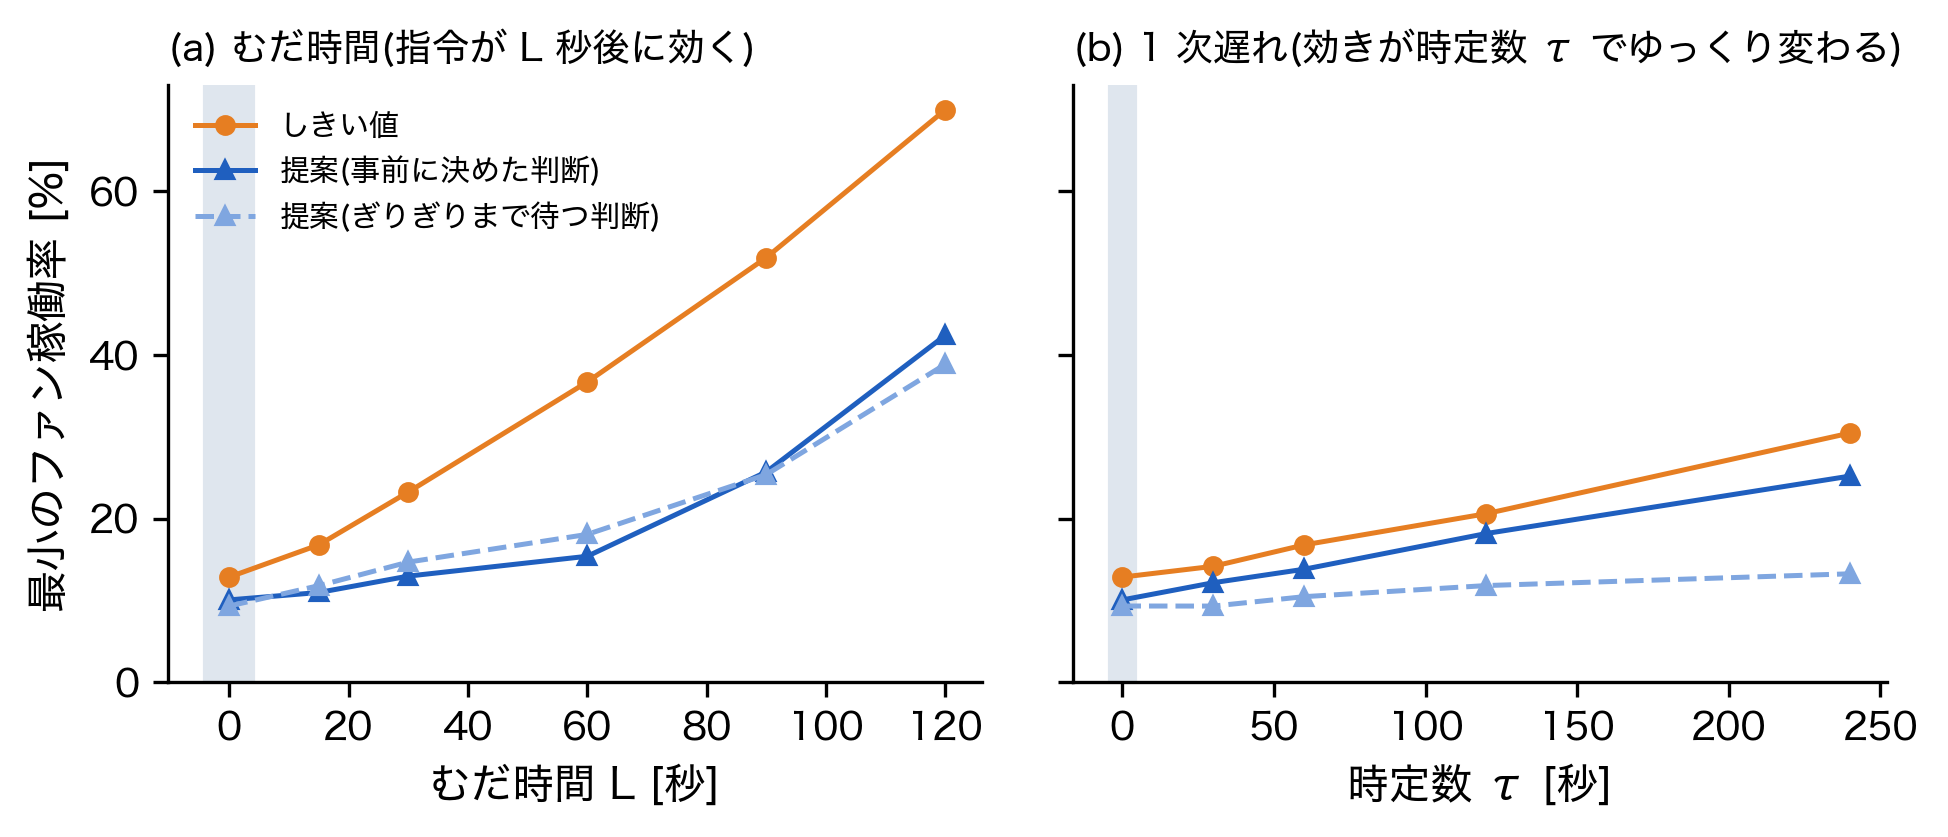
\includegraphics[width=\linewidth]{fig_slow_cooling.png}
  \caption{冷却の効きの遅れと、80\,℃ を超えない中での最小のファン稼働率(シミュレーション、4 パターンの平均)。灰色の帯は本研究の PoE+ HAT のファンに当たる。むだ時間 120 秒では、どの方式でも超過を避けられないパターン1本を除いた平均}
  \label{fig:eval-slow}
\end{figure}

\section{まとめ}\label{sec:eval-summary}
本章の結果をまとめる。

\begin{itemize}
  \item RQ1:ラックに並べた本研究の環境では、空間熱干渉はほぼ生じない(同定した $c$ は 0 に近く、符号も一定でない)
  \item RQ2:負荷とファンが変わらない区間では、30 秒先を MAE 約 0.7\,℃ で予測できる。誤差の大半は 30 秒以内の負荷の切り替えから生じる。干渉がないため、提案手法の $\sigma$ は一定となり、動的マージンは固定マージンと同じ働きになる
  \item RQ3:予測に基づく制御は 80\,℃ を超えずに、常時 ON と比べてファンの稼働を 55〜62\% 減らした。ただし、しきい値方式との差はほぼなかった
  \item 冷却の効きを遅くしたシミュレーションでは、むだ時間 15〜30 秒から、予測を用いる方式がしきい値方式より少ない稼働で 80\,℃ を守れるようになった。1次遅れでは、予測の使い方(判断の仕方)によって結果が変わり、「ぎりぎりまで待つ」判断で差が出た(新しい負荷のパターンでも確認)
\end{itemize}

提案手法がしきい値方式と差がなかった理由は第\ref{chap:discussion}章で考察する。
